\documentclass[10pt,conference]{IEEEtran}

\usepackage{latexsym,amsmath,amssymb,amsfonts,epsfig,subfigure, algorithmicx, algorithm, algpseudocode}

\newcommand{\real}{\mathbb{R}}
\newcommand{\nat}{\mathbb{N}}
\newcommand\spar[1]{\vspace{1ex}\noindent{\bf #1}}
\newcommand{\at}[1]{{{\it AT: #1}}}
\newcommand\T{\rule{0pt}{2.6ex}}
\newcommand\B{\rule[-1.2ex]{0pt}{0pt}}
\newcommand\C[1]{\multicolumn{1}{c}{#1}}
\newcommand\cspace{\vspace{2ex}} % correction space for tables
\newcommand\cfspace{\vspace{1.5ex}} % correction space for figures

\newcommand{\vmargin}[1]{\marginpar{\color{blue}\footnotesize [VI]: #1}}
\newcommand{\vtxt}[1]{{\color{red} #1}}

\begin{document}

\title{Next Steps for JHU Testbed design}

\author{
\IEEEauthorblockN{Jong Hyun Lim}
\IEEEauthorblockA{Department of Computer Science\\
Johns Hopkins University\\
Baltimore, MD\\
Email: ljh@cs.jhu.edu}
}

\maketitle

\begin{abstract}
\end{abstract}
\begin{figure}[t]
  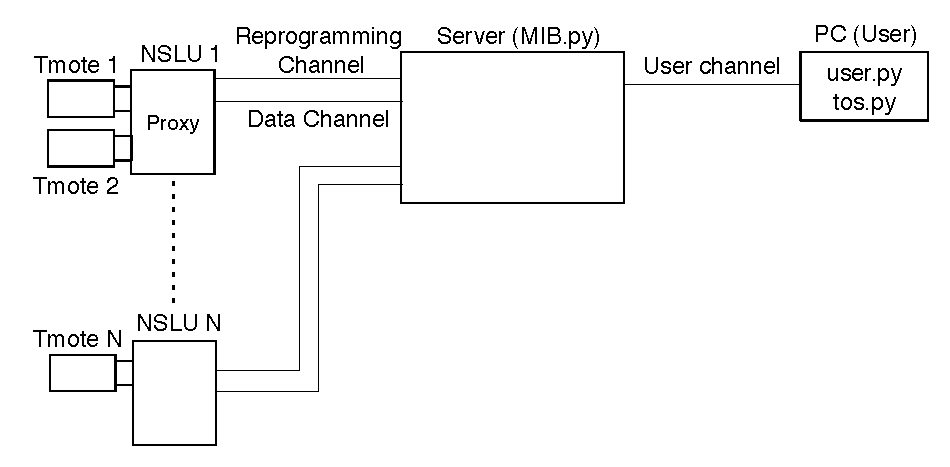
\includegraphics[width=.45\textwidth]{./figs/arch.eps}
  \caption{
  The architecture of new testbed, which consists of three main components:
  NSLU, server, user program.  Ultimately, the main goal of new testbed design
  is to enable a user to utilize the network communication capability of
  \textit{tos.py}.
  }
  \label{fig:arch}
\end{figure}

\section{Terminology}
This section introduces crucial terms used in this paper.\\
$\bullet$ \textbf{NSLU}: an embedded device~\cite{NSLU} manufactured by Cisco.
It uses Intel Ixp400 and has two USB connections.  In addition, it runs
\textit{Kamikaze 8.x} for its operating system, which is a modified version of
\textit{Openwrt} project~\cite{openwrt}.\\
$\bullet$ \textbf{Remote Mote}: a mote directly connected to NSLU. \\
$\bullet$ \textbf{Proxy}: a program running on a NSLU box. It reads and writes 
data to and from a remote mote or users. \\
$\bullet$ \textbf{MIB.py}: a program running on a server. It handles data 
to and from each mote and user. Once it receives data from a mote it logs
data. In addition, it manages connectivity with remote motes or users. \\

\section{Design Goal}
The main design goal of this project is to utilize existing
\textit{tos.py}~\cite{tos.py} for network communication in a tested.  By doing
so brings about two key benefits: $1)$ a user can use \textit{tos.py} to read
and write data to and from a remote mote as if the user uses to do with a mote
directly connected to his or her serial cable.  In other words, the user does
not need any special programs to communicate with the remote motes (only
tos.py).  $2)$ It simplifies proxy program by getting rid of serial
communication modules (e.g.  CRC check and formatting a user data into a AM
packet).  Previously, a proxy program was integrated with C serial libraries
provided by TinyOS 2.x, called serial forwarder.  On the other hand, in new
design these serial operations are now being taken care of by \textit{tos.py}
on user side.  Therefore, the proxy program only reads and writes data stream
to and from it with simple C read and write functions.

\section{Architecture} \label{sec:arch}
The testbed consists of three main components: $1)$ NSLU running proxy program, 
$2)$ server running \textit{MIB.py}, and PC running \textit{tos.py} as shown 
in Figure~\ref{fig:arch}. 

\spar{NSLU running proxy program.} The proxy program receives serial data from
a mote and sends it to server.  Similiarly, it receives data sent from a
server, which originates from a user, and delivers it to a mote.  As its name
suggests, It only works as a proxy so that it handles only data stream to and
from it.  In other words, it never interprets incoming or outing data to and from it.
In consequence of it, the implementation of the proxy becomes simple, which is
just read and write data with C functions.

Executing a proxy program is fully automatic.  As we know already, each NSLU
box has two USB ports.  If you connect a Tmote into one of the USB port, a
script pre-installed recognizes both MAC address of the Tmote and USB port to
which it is connected(e.g.  M4AN1DBY and /dev/ttyUSB0, respectively).  Then,
the proxy program tries to connect to a server(server address is also given in
the script) with known TCP port, and delivers the MAC of the Tmote.  Once the
server accepts the connection , it knows IP address and port number of the NSLU
box and MAC of the Tmote as well.  The tuple(IP, TCP port, MAC) makes it
possible to uniquely identifies each Tmote.  This opened channel is called
\textit{reprogramming channel} as Figure~\ref{fig:arch} shows.  It is not only
used for reprogramming, but also for sending keep-alive messages regularly to
the server.  This enable the server to monitor if a connection is still alive.

The proxy program creates another channel for data communication.  This is
because the proxy only processes stream of data so that the reprogramming
channel cannot be shared with data channel.  Specifically, the proxy cannot
distinguish between the image for reprogramming and data sent from user.  As a
result, the server maintains two separate channels for each Tmote in the
network.

\spar{Server running \textit{MIB.py}.} We run our python program MIB.py in a
server.  The main tasks of program are two-fold: $1)$ maintaining
connections(i.e channels) from NSLU boxes and users and $2)$ processing and
logging data from motes and users.  When the server accepts connections from
proxy program, it maintains two separate connections.  From this point on, the
server listens to the connection from a user (for sending and reciving data to
and from this mote or for reprgoramming).  If a mote sends data to server, the
server, by default, logs the data locally.  Additionally, if user channel is
opened, it sends the data to the user through user channel.

\spar{PC running \textit{user.py}.} One of the design goal of this new testbed
is not to change the way we use \textit{tos.py} on user's side.  The user's
python script, called \textit{user.py}, imports \textit{tos.py} provided by
TinyOS $2$.  The \textit{tos.py} provides separate interfaces to access to a
mote connected through serial or network.  To follow \textit{tos.py}'s
convention to connect to a remote mote, we need to specify the server IP or
host name with TCP port nubmer as following:
\begin{equation}
\label{eqn:mute}
\small
./user.py \hspace{1.5mm} network@mute.isi.jhu.edu:17003
\end{equation}
However, as we do not know to which TCP port a proxy program running on NSLU
box is assigned, we follows pre-defened rule to make this access feasible.
Even though we know IP and port number of NSLU box, it is time-consuming and
cumbersome to change IP or DNS name every time when we connect to different
mote in different NSLU boxes.  Therefore, we only specify the server's IP or
DNS name(which is constant) when a user want to connect to a mote, and use a
TCP port implying a mote's TOS\_NODE\_ID.  For this puropse, we use TCP port
number $17xxx$.  Specifically, we exploit the last three digits of the TCP
ports to imply TOS\_NODE\_ID.  For example, if a NSLU box has a mote
precompiled with TOS\_NODE\_ID $3$, we use TCP port number $17003$ to read and
write data to and from this mote.  As what a user suggests is mere
TOS\_NODE\_ID, the server needs to know which MAC address of a mote is
corresponding to this TOS\_NODE\_ID.  In the following subsection, we describe
the map file.

\subsection{Making Map file} \label{sec:map} When it comes to send and receive
data to and from NSLU boxes, a server needs to know to which mote it sends data
or from which mote it receives data.  As a NSLU box has two USB ports, IP
address cannot be used to distinguish each mote connected to that box.  A
simple and unique identifier is a mote's MAC address.  Before you run
\textit{MIB.py}, you need to manually make a file containing two columns.  The
first column specifies MAC addresses of each mote, and the second is
TOS\_NODE\_ID you want to translate to.  For example, if a use tries to send
data to mote $3$ by specifying \textit{network@mute.isi.jhu.edu:17003}, server
which listen to this port $17003$ looks up the MAC address corresponds to, and
by using the MAC it sends user's data to IP address and port number of
appropriate NSLU box, which is bound to one of the two motes.

\section{Instruction Manual}

\subsection{Installation.} \label{sec:install}To be able to use this testbed
program, you need to install the following programs in three components.

\spar{1. NSLU}\\
$1)$ If you want to connect Tmotes to NSLU, you first need to install USB
serial components(only if you do not have them).  If you have it, go to step
$2)$; otherwise, copy \textit{kmod-usb-serial-2.6.26.8-ixp4xx-1-armeb.ipk} and
\textit{kmod-usb-serial-ftdi-2.6.26.8-ixp4xx-1-armeb.ipk} and install the two
packages with the following command: \\

ipkg -i kmod-usb-serial-2.6.26.8-ixp4xx-1-armeb.ipk \\

ipkg -i kmod-usb-serial-ftdi-2.6.26.8-ixp4xx-1-armeb.ipk\\\\
$2)$ In this step, you install proxy program and a monitoring script.  The
monitoring script called \textit{telos-monitor} periodically check if a Tmote
is connected or not.  If it recognizes a Tmote, it automatically run proxy
program with parameters it collects through hotplug(the program fetches 
the MAC address of the Tmote). The installation process is the same as step $1)$. 
Install the package with ipkg command: \\

ipkg -i tinyos-telos-monitor-2.1-1-armeb.ipk \\\\
$3)$ The last step is to install \textit{cppbsl} for reprogramming. The method is the
same as previous steps: \\

ipkg -i tinyos-cppbsl-2.1-1-armeb.ipk\\\\
$4)$ If you want to flash your NSLU box with new image shipped with all the
components from step $1)$ to $3)$, follow the instruction provided by NSLU
webpage~\cite{NSLU}.  For this purpose, we provide a binary image file called
\textit{openwrt-nslu2-squashfs.bin}.

\spar{2. Server}\\
$1)$ Make sure you have a \textit{map} file in the directory where you want to 
run server program. To make this file, please refer Section~\ref{sec:map}\\\\
$2)$ In the server that monitors all the NSLU boxes, you just simply run
\textit{MIB.py} script in the directory you want.  The \textit{MIB.py} program
logs all the data it receives from NSLUs in \textit{./logs/current}.  If you
quit and rerun the program, previous \textit{current} file will automatically
be renamed as in \textit{UNIX time.incomplete}, e.g.
\textit{1258257773.1021.incomplete}.  Then, the \textit{MIB.py} generates new
\textit{current} file for the new run.

\spar{3. Your PC}\\
The following three files are used only for reprogramming motes. For read and 
write data from please read Section~\ref{sec:prereq} to~\ref{sec:write} \\\\
$1)$ server.extra:  This file specifies the IP address and port number where
the \textit{MIB.py} is located.  The location of the file should be
\$TOSROOT/support/make in your local computer.  To be able to use it, however,
a user needs to replaces the server address part of the file with your server
address.  Currently, the line containing server address is \textit{nc
mute.isi.jhu.edu 16462}.  Replace the server name with your server name or IP
address.  In addition, you also need to change the statement \textit{PROGRAM =
mute}. \\\\
$2)$ burn script: Having moved the server.extra file in the directory specified, 
copy the burn script into the directory containing your TinyOS application program. 
If you open up the file, you will see the following line 
\[
make\hspace{2.0mm} telosb\hspace{2.0mm} reinstall,\$i\hspace{2.0mm} mute,\$MAP
\]
Then, change the fifth column \textit{mute} to \textit{server}. By doing so, 
the burn script refer the \textit{server.extra} file while it reinstalls. 
Once you modifies the file, running the script is the same as we do for any
other bash script. \\\\
$3$ map file: The file consists of two columns: the first column specifies
the MAC address of each mote in testbed and the second TOS\_NODE\_ID with which
you want to compile the mote.  The burn scipt reads this file when it comes to
reprogram mote.  Currently in the burn script, the location of the all file is
set to be located in your home directory. In addition, this file should be the 
same as the server's map file. 

\subsection{Prerequisite to reading and writing.} 
\label{sec:prereq}

Suppose a user writes a python
script(called \textit{user.py}) to read and write a data from a remote
mote.  The first step is to import \textit{tos.py} provided by TinyOS 2.x as
following:
\[
import \hspace{1.2mm} tos 
\]
After this, the user script would need the following statement to initiate 
network(or serial) communiation: 
\[
am = tos.AM()
\]
Having written this statement, the user's read and write operations will be
done through AM's read and write functions by calling either \textit{am.read()}
or \textit{am.write()}.

In contrary to serial data communication, where we specify the serial port,
such as /dev/ttyUSB0, we specify instead the TCP port number to connect to a
particular mote.  For example, if we want to connect to a remote mote $3$, as
defined in numbering scheme in Section~\ref{sec:numbering}, we specify the TCP
port as $17003$.  Overall, by following the \textit{tos.py}'s convention for
network connection, the user script program will be run as following: 
\begin{equation}
\label{eqn:command}
\small
./user.py \hspace{1.5mm} network@mute.isi.jhu.edu:17003
\end{equation}
where \textit{mute.isi.jhu.edu} is the server running the MIB.py program.

\subsection{Reading Data from a Mote}
Reading data from a mote is simple.  If a user wants to read data continuously,
the \textit{user.py} should contain the following statements as we do for serial 
communication:
\begin{algorithm}
\caption{user.py}\label{user.py}
\begin{algorithmic}
  \State While True:
    \State \hspace{5.2mm}p = am.read()
    \State \hspace{5.2mm}print p.data
  \State ...
\end{algorithmic}
\end{algorithm}

\subsection{Writint Data to a Mote}\label{sec:write}
For writint data to a mote, a user first needs to build a packet formatted in a
serial ActiveMessage(called AM packet for short).  For details about how to
build the the AM packet, reader should refer~\cite{tos.py}.  We assume that a
user has built an AM packet using classes provided by \textit{tos.py}.  We call
the user's packet as \textbf{ampacket}.  If this is the case, the user script
will contain the following line:
\[
if\hspace{1.2mm} am.write(ampacket, 238) == True: \cdots
\]
With this command executed, \textit{tos.py} sends \textbf{ampacket} to a mote
$3$ with AM ID $238$, and waits for an acknowledgement.  It ack is received
successfully, the write function returns \textit{True}.

\subsection{Reprogramming a Mote}
To reprogram motes installed in a testbed, first make sure that you have the
files ready mentioned $3) \hspace{1.2mm}Your \hspace{1.2mm}PC$ in
Section~\ref{sec:install}. If ready, just run the burn script in the directory 
where your TinyOS $2.x$ program is located. 

\section{Future work}
Currently, reprograming an Epic mote connected to an open-mesh is not
implemented.  We will focus on this to make repgoramming on Epic possible.

\section*{Acknowledgment}
First of all, i would like thank Razvan Musaloiu-E of HiNRG at JHU for his
tremendous support.  The server program is based on the his first version.
Additionally, the burn script and server.extra files are also written by him.

\begin{thebibliography}{1}

\bibitem{NSLU}
``NSLU2-Linux,'' \emph{http://www.nslu2-linux.org/wiki/}. 

\bibitem{openwrt}
``OpenWrt: wireless freedom,'' \emph{http://www.openwrt.org/}. 

\bibitem{tos.py}
``tos.py - TinyOS Documentation Wiki,'' \emph{http://docs.tinyos.net/}. 

\end{thebibliography}

% that's all folks
\end{document}
